\documentclass[a4paper, 11pt]{article}

%Math
\usepackage{amsmath}
\usepackage{amsfonts}
\usepackage{amssymb}
\usepackage{amsthm}
\usepackage{ulem}
\usepackage{stmaryrd} %f\UTF{00FC}r Blitz!

%PageStyle
\usepackage[ngerman]{babel} % deutsche Silbentrennung
\usepackage[ansinew]{inputenc} % wegen deutschen Umlauten
\usepackage{fontenc}
\usepackage{fancyhdr, graphicx} %for header/footer
\usepackage{wasysym}
\usepackage{fullpage}
\usepackage{textcomp}

% Listings
\usepackage{color}
\usepackage{xcolor}
\usepackage{listings}
\usepackage{caption}

% Code listenings
\DeclareCaptionFont{white}{\color{white}}
\DeclareCaptionFormat{listing}{\colorbox{gray}{\parbox{\textwidth}{#1#2#3}}}
\captionsetup[lstlisting]{format=listing,labelfont=white,textfont=white}
 
\lstdefinestyle{JavaStyle}{
 language=Java,
 basicstyle=\footnotesize\ttfamily, % Standardschrift
 numbers=left,               % Ort der Zeilennummern
 numberstyle=\tiny,          % Stil der Zeilennummern
 stepnumber=5,              % Abstand zwischen den Zeilennummern
 numbersep=5pt,              % Abstand der Nummern zum Text
 tabsize=2,                  % Groesse von Tabs
 extendedchars=true,         %
 breaklines=true,            % Zeilen werden Umgebrochen
 frame=b,         
 %commentstyle=\itshape\color{LightLime}, Was isch das? O_o
 %keywordstyle=\bfseries\color{DarkPurple}, und das O_o
 basicstyle=\footnotesize\ttfamily,
 stringstyle=\color[RGB]{42,0,255}\ttfamily, % Farbe der String
 keywordstyle=\color[RGB]{127,0,85}\ttfamily, % Farbe der Keywords
 commentstyle=\color[RGB]{63,127,95}\ttfamily, % Farbe des Kommentars
 showspaces=false,           % Leerzeichen anzeigen ?
 showtabs=false,             % Tabs anzeigen ?
 xleftmargin=17pt,
 framexleftmargin=17pt,
 framexrightmargin=5pt,
 framexbottommargin=4pt,
 showstringspaces=false      % Leerzeichen in Strings anzeigen ?        
}

%Config
\renewcommand{\headrulewidth}{0pt}
\setlength{\headheight}{15.2pt}
\pagestyle{plain}

%Metadata
\title{Algorithmen \& Datenstrukturen 2}
\author{Jan F�ssler}
\date{3. Semester (HS 2012)}
\fancyfoot[C]{If you use this documentation for a exam, you should offer a beer to the authors!}

% hier beginnt das Dokument
\begin{document}

% Titelbild
\maketitle
\thispagestyle{fancy}

\newpage

% Inhaltsverzeichnis
\pagenumbering{Roman}
\tableofcontents	  	


\newpage
\setcounter{page}{1}
\pagenumbering{arabic}

% Inhalt Start

\section{Listen}
Eine verkettete Liste (linked list) ist eine dynamische Datenstruktur zur Speicherung von Objekten. Sie eignen sich f�r das speichern einer unbekannten Anzahl von Objekten, sofern kein direkter Zugriff auf die einzelnen Objekte ben�tigt wird. Jedes Element in einer Liste muss neben den Nutzinformationen auch die notwendigen Referenzen zur Verkettung enthalten.\\ 
Es gibt drei verschiedene Arten von Listen:\\
\begin{center}
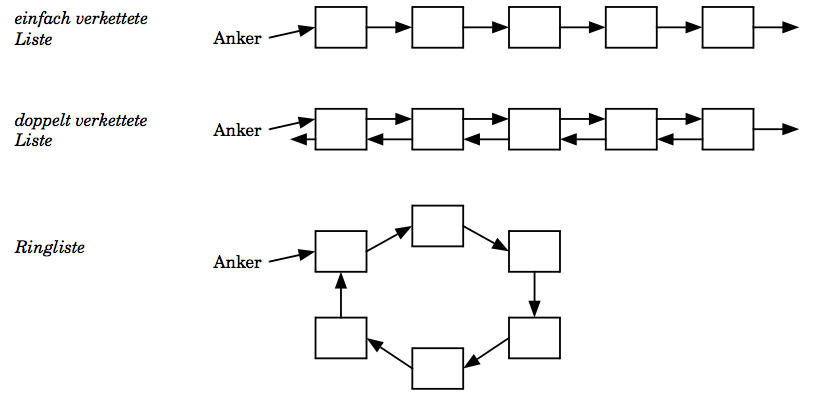
\includegraphics[scale=0.4]{listen.png}
\end{center}

\lstinputlisting[language=java,caption=einfache Linked List,style=JavaStyle]{linked_list.java}


\subsection{Stack}
Der Stack ist eine dynamische Datanstruktur bei der man nur auf das oberste Element des Stabels zugreifen (top), ein neues Element auf den Stabel legen (push) oder das oberste Element des Stapels entfernen (pop) kann.
\lstinputlisting[language=java,caption=Implementierung eines Stacks,style=JavaStyle]{stack.java}

\subsection{Erweiterte Liste}
Dies ist mal eine m�gliche und vor allem nur teilweise Implementierung einer doppelt verlinkten Liste. Die Implementierung des Iterators und der sortierung sind ausgeklammert in Unterkapitel.
\lstinputlisting[language=java,caption=Liste mit Iterator,style=JavaStyle]{advanced_list.java}

\subsubsection{Iterators}
Die Schnittstelle java.util.Iterator, erlaubt das Iterieren von Containerklassen. Jeder Iterator stellt Funktionen namens next(), hasNext() sowie eine optionale Funktion namens remove() zur Verf�gung. Der folgende ListIterator stellt auch noch Funktionen f�r r�ckwertsiterieren zur Verf�gung, sowie die M�glichkeit den aktuellen Index abzufragen. Zudem kann damit noch direkt �ber den Iterator Elemente eingef�gt oder ersetzt werden.

\lstinputlisting[language=java,caption=Iterators,style=JavaStyle]{linked_list_iterators.java}

\subsubsection{Merge Sort}
\lstinputlisting[language=java,caption=Merge Sort,style=JavaStyle]{linked_list_mergesort.java}

\subsection{Skip-Liste}
Die Skip-Liste ist eine sortierte, einfach verkettete Liste, die uns aber ein schnelleres Suchen von Elementen in der Datenstruktur erlaubt. In einer sortierten, verketteten Liste m�ssen wir jedes Element einzeln durchlaufen bis wir das gew�nschten Element gefunden haben. Wenn wir nun aber in der sortierten Liste auf jedem zweiten Element eine zus�tzliche Referenz auf zwei Elemente weiter hinten setzen, dann reduziert sich die Anzahl zu besuchender Elemente auf einen Schlag um rund die H�lfte. Genau betrachtet mu?ssen wir nie mehr als $(n/2) + 1$ Elemente besuchen (n ist die L�nge der Liste). 
\begin{center}
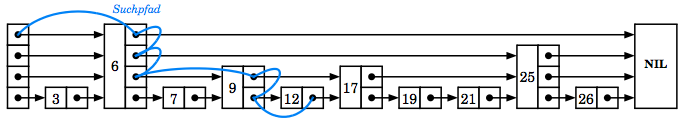
\includegraphics[scale=0.65]{skip_liste.png}
\end{center}
\subsubsection{Suchen}
Um ein Element zu finden, gehen wir so lange auf dem momentanen Level den Referenzen entlang, wie das zu suchende Element immer noch gr�sser ist als das gerade aktuelle. Geht es auf dem momentanen Level nicht mehr weiter, gehen wir einfach einen Level tiefer und suchen wie beschrieben weiter. Wenn wir auf Level 0 nicht mehr weiterkommen, m�ssen wir gerade vor dem gesuchten Element sein, oder es gibt dieses Element gar nicht.
\subsubsection{Einf�gen}
Um ein Element einzuf�gen, gehen wir genau gleich wie beim Suchen vor. Zus�tzlich f�hren wir aber noch ein Array update mit, in dem all jene Elemente gespeichert werden, auf denen wir einen Level- Wechsel vorgenommen haben. Endet die Suche, haben wir entweder ein Element mit gleichem key gefunden und ersetzen es, oder wir haben den Ort gefunden, wo wir unser Element einf�gen wollen. Beim Einf�gen bestimmen wir zuerst den zuf�lligen Level des neuen Elementes. Danach setzen wir alle Referenzen des neuen Elementes so, dass sie dorthin zeigen, wo die Elemente in unserem update-Array hinzeigen. Zum Schluss mu?ssen wir bloss noch die Referenzen der Elemente im update-Array auf das neue Element umbiegen.
\subsubsection{Entfernen}
Wiederum gehen wir genau gleich wie beim Suchen vor. Auch diesmal f�hren wir zusa?tzlich noch ein Array update mit, in dem all jene Elemente gespeichert werden, auf denen wir einen Level-Wechsel vorgenommen haben. Da wir in der Skip-Liste einen MaxLevel haben, ist die L�nge des Arrays MaxLevel + 1. Ist das zu entfernende Element gefunden, m�ssen wir alle Referenzen umbiegen, die auf dieses Element gerichtet sind. Dazu gehen wir unser update-Array durch und biegen alle Referenzen so um, dass sie dorthin zeigen, wo unser zu entfernendes Element hinzeigt. Danach k�nnen wir das zu entfernende Element einfach aus der Liste entnehmen.

% Inhalt Ende
\end{document}